\documentclass[hidelinks]{article}

%% Deutsche Silbentrennung und Sprache (neue Rechtschreibung)
\usepackage[english]{babel}
%% Verwende Umlaute direkt
\usepackage[utf8x]{inputenc}
%% Hyperlinks für interne Referenzen
\usepackage{hyperref}
%% Grafiken einbinden
\usepackage{graphicx}
\usepackage{float}
%% Paket für Unterabbildungen pro Abbildung
\usepackage{subfig}

\usepackage{forloop}

\usepackage{enumerate}
\usepackage{amsmath}
\usepackage{amssymb}
\usepackage{algorithm}
\usepackage[noend]{algpseudocode}
\newcommand\Let[2]{\State #1 $\gets$ #2}
\algrenewcomment[1]{\(\qquad \triangleright\) #1}
\newcommand\Blet[2]{\State \textbf{let} #1 \textbf{be} #2}

\usepackage{mathtools}
% Proof system
\usepackage{amsthm}

\theoremstyle{plain}
\newtheorem{thm}{Theorem}[section]
\newtheorem{lem}[thm]{Lemma}

\theoremstyle{definition}
\newtheorem{defn}[thm]{Definition}
\newtheorem{bsp}[thm]{Example}

\newtheoremstyle{rem} % name
    {\topsep}                    % Space above
    {\topsep}                    % Space below
    {}                   % Body font
    {}                           % Indent amount
    {\bf}                   % Theorem head font
    {:}                          % Punctuation after theorem head
    {.5em}                       % Space after theorem head
    {}  % Theorem head spec (can be left empty, meaning ‘normal’)

\theoremstyle{rem}
\newtheorem*{remark}{Note}

%\usepackage{xpatch}
%\makeatletter
%% Remove last point from definitions, theorems, etc.
%\xpatchcmd{\@thm}{\thm@headpunct{.}}{\thm@headpunct{\\}}{}{}
%\makeatother

% Seitenränder
%TODO originally 1.5 in
\usepackage[margin=1.3in]{geometry}
% Zitate
\usepackage{cite}
% Tabellen
\usepackage[table]{xcolor}

% Graphs
\usepackage{tikz}
\usetikzlibrary{calc,arrows.meta,positioning}
\usepackage{tikz-3dplot}
\usepackage{pgfplots}

\setlength{\parindent}{0pt}

% Titel der Arbeit
\title{Power management - Dynamic Programming}
% Angaben zum Author
\author{Kevin Kappelmann\\
  \multicolumn{1}{p{.7\textwidth}}{\centering\emph{Chair for Theoretical Computer Science,\\
  Technical University of Munich}}}  

\pagestyle{plain}

%------------------------------------------------------------------------------
\begin{document}

\pagenumbering{arabic}

\begin{sloppypar}
Requirements:
\begin{itemize}
	\item Convex cost function $f$
	\item Power down costs are w.l.o.g.\ equal to 0.
	\item $\lambda_0=\lambda_T=0$
	\item $\forall t\in[T-1]:\lambda_t\in[0,2]$
	\item All servers are powered down at $t=0$ and $t=T$.
\end{itemize}
Input:
\begin{itemize}
	\item $\beta$: Power up costs.
	\item $\lambda_1\ldots\lambda_{T-1}$: Arrival rates
\end{itemize}
We construct a directed acyclic graph as follows:\\
For each timestep $t\in[T-1]$ we vertices $(t,0),(t,1)$ and $(t,2)$ modelling the number of active servers at time t. Furthermore, we add vertices $(0,0)$ and $(T,0)$ for our initial and final state respectively.\\
In order to warrant that $\forall t\in[T-1]$ there are at least $\lceil\lambda_t\rceil$ active servers, we define an auxiliary function which calculates the costs for handling an arrival rate $\lambda$ with $x$ active servers:
\begin{equation}
	c(x,\lambda)\coloneqq\begin{cases}
	  x*f(\lambda/x), & \text{if $\lambda\le x$}\\
	  \infty, & \text{otherwise}
	  \end{cases}
\end{equation}
Then, $\forall t\in[T-2],i,j\in\{0,1,2\}$ we add edges from $(t,i)$ to $(t+1,j)$ with weight
\begin{equation}
	d(i,j,\lambda_{t+1})\coloneqq\underbrace{\beta*\min\{0,j-i\}}_{\text{power up costs}}+c(j,\lambda_{t+1})
\end{equation}
Finally, $\forall i\in\{0,1,2\}$ we add edges from $(0,0)$ to $(1,i)$ with weight $d(0,i,\lambda_1)$ and from $(T-1,i)$ to $(T,0)$ with weight 0.
\begin{figure}[H]
\centering
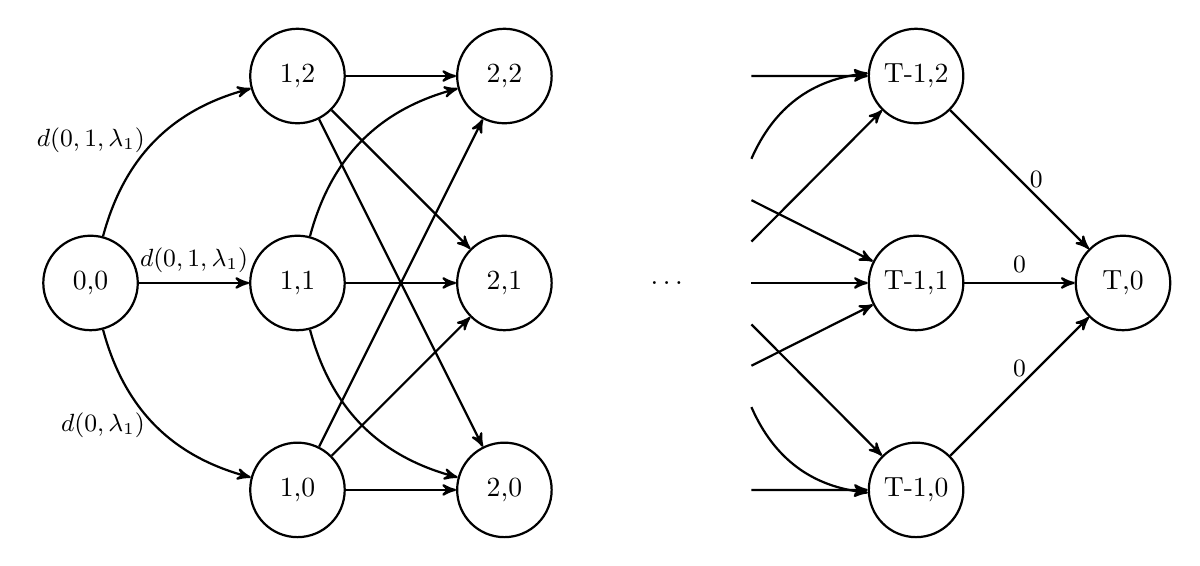
\begin{tikzpicture}[->,>=stealth',auto,node distance=1.4cm,thick,node/.style={minimum size=1.2cm,circle,draw}]

  \node[node] (1) {0,0};
  \node[node] (3) [right =of 1] {1,1};
  \node[node] (2) [above =of 3] {1,2};
  \node[node] (4) [below =of 3] {1,0};
  \node[node] (6) [right =of 3] {2,1};
  \node[node] (5) [above =of 6] {2,2};
  \node[node] (7) [below =of 6] {2,0};
  \node[node] (9) [right =4cm of 6] {T-1,1};
  \node[node] (8) [above =of 9] {T-1,2};
  \node[node] (10) [below =of 9] {T-1,0};
  \node[node] (11) [right =of 9] {T,0};

  \node at ($(6)!.4!(9)$) {\ldots};

  \path[every node/.style={font=\sffamily\small}]
    (1) edge [bend left] node[left] {$d(0,1,\lambda_1)$} (2)
        edge node[above] {$d(0,1,\lambda_1)$} (3)
	edge [bend right] node[left] {$d(0,\lambda_1)$} (4)
    (2) edge (5)
        edge (6)
	edge (7)
    (3) edge [bend left] (5)
        edge (6)
	edge [bend right] (7)
    (4) edge (5)
        edge (6)
	edge (7)
    (8) edge node[right] {$0$} (11)
    (9) edge node[above] {$0$} (11)
    (10) edge node[above] {$0$} (11);
   \path [->,draw,thick] ($(5)!.6!(8)$) to (8);
   \path [->,draw,thick] ($(5)!.6!(9)$) to (9);
   \path [->,draw,thick] ($(5)!.6!(10)$) to (10);
   \path [->,draw,thick] ($(6)!.6!(8)$) to [bend left] (8);
   \path [->,draw,thick] ($(6)!.6!(9)$) to (9);
   \path [->,draw,thick] ($(6)!.6!(10)$) to [bend right] (10);
   \path [->,draw,thick] ($(7)!.6!(8)$) to (8);
   \path [->,draw,thick] ($(7)!.6!(9)$) to (9);
   \path [->,draw,thick] ($(7)!.6!(10)$) to (10);

\end{tikzpicture}
\caption{All edges from $(t,i)$ to $(t+1,j)$ have weight $d(i,j,\lambda_{t+1})$}
\end{figure}

\begin{algorithm}[H]
    \caption{Optimal schedule for $m=2$ homogeneous servers}
    \begin{algorithmic}[1]
        \Require{Convex cost function $f$, $\lambda_0=\lambda_T=0$, $\forall t\in[T-1]:\lambda_t\in[0,2]$}
   \Function{schedule}{$T,\beta,\lambda_1,\ldots,\lambda_{T-1}$}
	\If{$T<2$}
		\State \Return
	\EndIf
	\Blet{$p[2\ldots T-1,2]$ and $m[1\ldots T-1,2]$}{new arrays}
	\For{$j \gets 0 \textrm{ to } 2$}
		\Let{$m[1,j]$}{$d(0,j,\lambda_1)$}
	\EndFor
	\For{$t \gets 1 \textrm{ to } T-2$}
		\For{$j \gets 0 \textrm{ to } 2$}
			\Let{$opt$}{$\infty$}
			\For{$i \gets 0 \textrm{ to } 2$}
				\Let{$m[t+1,j]$}{$m[t,i]+d(i,j,\lambda_{t+1})$}
				\If{$m[t+1,j]<opt$}
					\Let{$opt$}{$m[t+1,j]$}
					\Let{$p[t+1,j]$}{$i$}
				\EndIf
			\EndFor
		\EndFor
	\EndFor
	\State \Return{$p$ and $m$}
  \EndFunction
  \end{algorithmic}
\end{algorithm}
\begin{algorithm}[H]
    \caption{Extract schedule for m=2 homogeneous servers}
    \begin{algorithmic}[1]
   \Function{Extract}{$p,m,T$}
	\Blet{$x[0\ldots T]$}{a new array}
	\Let{$x[0]$}{$x[T]\leftarrow 0$}
	\Let{$x[T-1]$}{$\underset{0\le i\le 2}{arg\ min}\{m[T-1,i]\}$}
	\For{$t \gets T-2 \textrm{ to } 1$}
		\Let{$x[t]$}{$p[t+1,x[t+1]]$}
	\EndFor
	\State \Return{$x$}
  \EndFunction
  \end{algorithmic}
\end{algorithm}


%\begin{proof}[Sketch for proof of correctness]
%We show that the algorithm calculates the correct costs and returns an optimal schedule $\forall T\in\mathbb{N}_{\ge 2}$ using induction.
%\begin{enumerate}
%\item[\textbf{Basis:}] For $T=2$ it holds $\lambda_0=\lambda_2=x_0=x_T=0$ and $\lambda_1\in(0,2]$. Therefore, the costs for the optimal schedule are $min\bigl\{f(\lambda_1)+\beta, f(\lambda_1/2)+2*\beta\bigr\}$. These costs are calculated at line 4-5 and minimized at line 18.\end{enumerate}
%\item[\textbf{Inductive step:}] Assuming the algorithm delivers a correct result for $T\in\mathbb{N}_{\ge 2}$, we show that it delivers a correct result for $T+1$.\\
%Firstly, we recognize that the executed statements of the algorithm for $T$ and $T+1$ are the same up to the last iteration of the for-loop at line 6. Hence, using the induction hypothesis, we can assume that $m_{1,\{1,2\}}$ up to $m_{T-1,\{1,2\}}$ are calculated correctly at this point.\\
%In order to calculate the minimum costs for using 1 machine at time T, we simply need to find $min\bigl\{m_{T-1,1},m_{T-1,2}\bigr\}+f(\lambda_T)$. This step is handled at line 7-8.\\
%In order to calculate the minimum costs for using 2 machines at time T, we need to find $min\bigl\{m_{T-1,1}+\beta,m_{T-1,2}\bigr\}+f(\lambda_T/2)$. This step is handled at line 9-16.\\
%Note: We do not need to consider possibilities where 2 servers are active but only 1 server is used. This follows from the convexity of $f$:
    %\begin{alignat*}{5}
        %f\Bigl(\frac{0+\lambda_t}{2}\Bigr)&=&f\Bigl(\frac{\lambda_t}{2}\Bigr)&\stackrel{convexity}{\le}\frac{f(0)+f(\lambda_t)}{2}\\
        %&\Leftrightarrow\quad&\underbrace{2*f\Bigl(\frac{\lambda_t}{2}\Bigr)}_{\text{using 2 servers}}&\quad\le\underbrace{f(0)+f(\lambda_t)}_{\text{2 active servers, using only 1}}
    %\end{alignat*}
%\end{proof}
\end{sloppypar}
\end{document}
